\documentclass[tikz,convert={density=300,size=300x300,outfile=\jobname.png}]{standalone}

\usetikzlibrary{automata,calc,trees,positioning,arrows,chains,shapes.geometric,%
decorations.pathreplacing,decorations.pathmorphing,shapes,%
matrix,shapes.symbols,plotmarks,decorations.markings,shadows}
\usepackage{amsmath}

\begin{document}
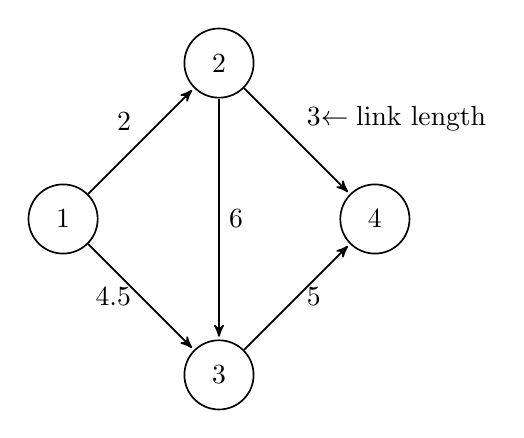
\begin{tikzpicture}[->,>=stealth',shorten >=1pt,auto,node distance=2.8cm,
                    semithick]

  \node[state] (node1) [] {1};
  \node[state] (node2) [above right of=node1] {2};
  \node[state] (node3) [below right of=node1] {3};
  \node[state] (node4) [below right of=node2] {4};

  \path (node1) edge node {2} (node2)
  		(node1) edge node [left] {4.5} (node3)
  		(node2) edge node {6} (node3)
  		(node2) edge node {3$\leftarrow\text{link length}$} (node4)
  		(node3) edge node [right] {5} (node4)
        ;
\end{tikzpicture}
\end{document}